\subsection{Authorization}
    \par
    The site is protected with the OAuth 2.0 token flow; users login using a central authorization server and receive a bearer token. The browser forwards this token in the header of subsequent request as the user visits each microservice. This token is validated by each service, providing a seamless login experience whilst maintaining security.

\subsection{Internal Communications}
    \par
    To maintain compatibility between the various microservices a common messaging protocol was selected. Building on the groups experience writing web applications, we chose to serialise messages into JSON and use REST endpoints. These APIs are then protected with the same OAuth 2.0 authorization flow as user facing pages, but instead rely on client credentials.

\subsubsection{nginx}
    \begin{figure}[H]
        \centering
        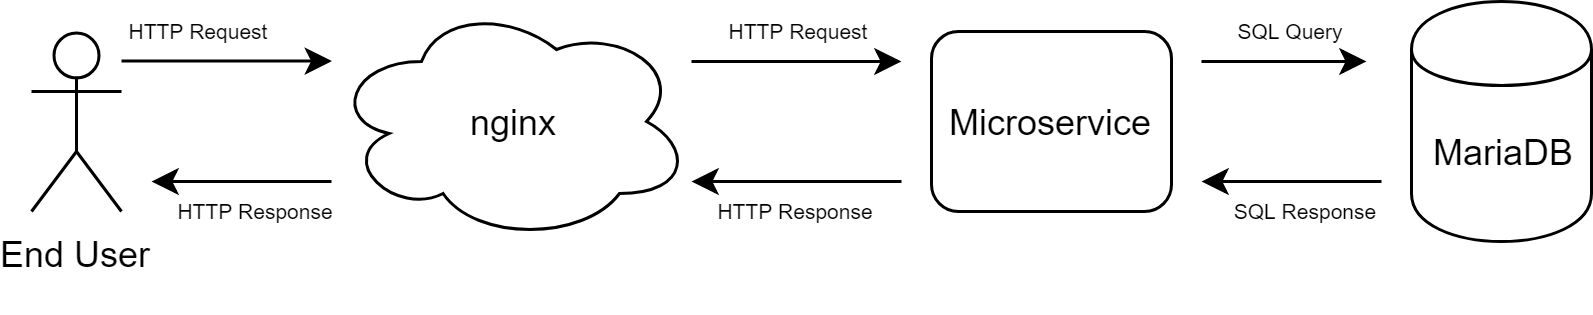
\includegraphics[width=\textwidth]{Images/nginx_proxy_flow.png}
        \caption{Traffic flow diagram showing an end user's browser connecting to the internet facing \textit{nginx} server, which then proxies requests through to the backend microservice}
    \end{figure}
    
    The Aber Fitness system architecture means that services are not exposed to the internet, but are instead available over an internal Docker network which allows containers to communicate with each other. In order to provide external access to the web servers of all of our microservices we have deployed nginx, an open-source and free web server which features highly customisable config files. Through the use of nginx's \lstinline{proxy\_pass} directive, we are able to take requests from end users and pass them through to the correct backend microservice based on the requested URI. \textbf{TODO: link figure above}
    

